\documentclass[a4paper,11pt]{article}
\usepackage{mathpazo}
\usepackage{tikz}
\usetikzlibrary{shapes}
\oddsidemargin -0.54cm
\textwidth 17.00cm
\textheight 24cm
\topmargin -1.3cm
\parindent 0pt
\parskip 1ex
\pagestyle{empty}
\begin{document}
\medskip\hrule\medskip

-40 0 -10 0 are inserted 

Width = 31
scale =0.548 

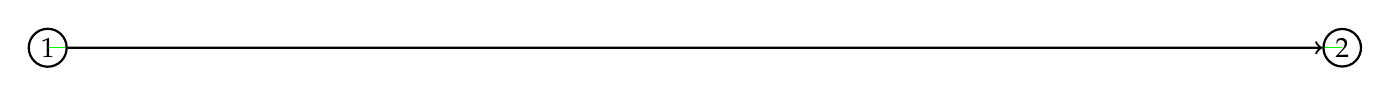
\begin{tikzpicture}[scale=0.548]
\draw [help lines, color=green] (-40,0) grid (-10,0);

\draw [thick] (-40,0) node[draw, rounded rectangle] (0) {1};
\draw [thick] (-10,0) node[draw, rounded rectangle] (1) {2};
\draw [->, thick] (0) to (1);

\end{tikzpicture}

\medskip\hrule\medskip
\end{document}